\documentclass[a4paper,12pt]{article}

\usepackage[utf8]{inputenc}
\usepackage[english,russian]{babel}
\usepackage{indentfirst}
\usepackage[unicode=true]{hyperref}

\usepackage{amsmath,amssymb,amsfonts,longtable,hhline}
\usepackage{mathrsfs}
\usepackage{multimedia} 

\usepackage{listings}
\usepackage{color}
\definecolor{codegreen}{rgb}{0,0.6,0}
\definecolor{codegray}{rgb}{0.5,0.5,0.5}
\definecolor{codepurple}{rgb}{0.58,0,0.82}
\definecolor{backcolour}{rgb}{1,1,1}

%Code listing style named "mystyle"
\lstdefinestyle{mystyle}{
  backgroundcolor=\color{backcolour},   commentstyle=\color{codegreen},
  keywordstyle=\color{magenta},
  numberstyle=\normalsize\color{codegray},
  stringstyle=\color{codepurple},
  basicstyle=\singlespacing\large,
  breakatwhitespace=false,         
  breaklines=true,                 
  captionpos=b,                    
  keepspaces=true,                 
  numbers=left,                    
  numbersep=5pt,                  
  showspaces=false,                
  showstringspaces=false,
  showtabs=false,                  
  tabsize=2
}

\lstset{style=mystyle}

\usepackage{geometry}
\geometry{left=2.5cm}
\geometry{right=1.5cm}
\geometry{top=2cm}
\geometry{bottom=2cm}

\usepackage{graphicx}
\usepackage{setspace}

\usepackage[labelsep=period]{caption}

\renewcommand{\baselinestretch}{1.5}
\makeindex
\graphicspath{{imgs/}}

\begin{document}
\large
\begin{titlepage}
    \newpage
    \begin{singlespacing}
        \begin{center}
            Министерство образования и науки Российской Федерации

            федеральное государственное бюджетное образовательное учреждение
            высшего образования \\
            «Иркутский государственный университет» \\
            (ФГБОУ ВО «ИГУ»)

            Институт математики, экономики и информатики

            Кафедра вычислительной математики и методов оптимизации

            % \flushright{Кафедра ВМиО}
            \vspace{5em}
            % \begin{center}
            %   \Large Численная аппроксимация множества достижимости импульсной
            %   управляемой системы 
            % \end{center}
            { \bf ВЫПУСКНАЯ КВАЛИФИКАЦИОННАЯ РАБОТА\\БАКАЛАВРА }
            \\[0.3cm]
            по направлению 01.03.02 Прикладная математика и информатика \\
            профиль Математическое и компьютерное моделирование

            \vspace{1em}

            { \Large Численная аппроксимация множества достижимости импульсной
            управляемой системы }
        \end{center}      
        \vspace{2em}

        \begin{flushright}
            {
                \parindent=0pt
                Студента 4 курса очного отделения\\
                группы 2422\\
                Апановича Данила Владимировича

                \vspace{1em}

                Руководитель:\\
                д. ф.-м. н., профессор кафедры\\ Вычислительной математики и Методов оптимизации \\ 
                \underline{\phantom{Четкая подпись}} Дыхта В.А. 

                \vspace{1em}

                Соруководитель:\\
                к.т.н., научный сотрудник ИДСТУ СО РАН\\
                \underline{\phantom{Четкая подпись}} Воронов В.А. 

                \vspace{1em}

                Допущена к защите:\\
                д. ф.-м. н., профессор кафедры\\ Вычислительной математики и Методов оптимизации \\ 
                \underline{\phantom{Четкая подпись}} Дыхта В.А. 

            }
        \end{flushright}

        \vspace{\fill}
        %    \vfill

        \begin{center}
            г.Иркутск --- 2016г.
        \end{center}

    \end{singlespacing}
\end{titlepage}

\tableofcontents
\pagebreak
\section*{Введение}
\addcontentsline{toc}{section}{Введение}
\label{intro}

Оценки множества достижимости управляемой системы, т.е. множества всех
состояний, в которые система может быть переведена из заданной начальной
точки за фиксированное время, играют важную роль как в теории динамических
систем, так и в некоторых прикладных задачах.  В частности, в задаче
оптимального управления с терминальным функционалом знание множества
достижимости позволяет найти значение задачи и конечную точку оптимальной
траектории как решение задачи математического программирования на множестве
достижимости. Знание множества достижимости делает тривиальным вопрос о
существовании допустимого управления в задаче с закрепленными концами (т.е.
об управляемости пары состояний).  В том случае, если задана конечная точка
траектории, аналогичным образом в обратном времени вычисляется множество
всех состояний, из которых можно перейти в заданное.  Поскольку множество
достижимости, как правило, не может быть найдено точно, используются
внутренние и внешние оценки, которые, соответственно, дают лишь
приближенный ответ в перечисленных выше задачах.

Оценка множества достижимости позволяет понять, как может вести себя
система, замкнутая по обратной связи, при неизвестных внешних
воздействиях (к примеру, действие ветра на самолет, управляемый
автопилотом), и позволяет определить, не выходят ли значения
переменных за грань допустимых.  Также можно привести в качестве
примера задачу уклонения самолета от выпущенной в него ракеты ---
здесь оценки множества достижимости характеризуют, с одной стороны,
начальные состояния, при которых ракета попадет в самолет при любой
его допустимой траектории; с другой стороны --- множество состояний,
при которых самолет гарантированно уклонится от ракеты.

Проблеме оценки множеств достижимости управляемых динамических систем,
описываемых системой обыкновенных дифференциальных уравнений,
посвящено большое количество работ.  Широко применяется аппарат
эллипсоидального исчисления, позволяющий находить как внутренние, так
и внешние оценки (А.Б. Куржанский, Ф.Л. Черноусько).  Известны также
методы, в которых оценки строят в виде многогранников (в частности,
параллелепипедов).  Принципиально другой подход основан на методе
динамического программирования Р.Беллмана: множество достижимости
рассматривается как поверхность уровня функции цены.

В управляемых системах возможны ситуации, когда за короткий период
времени происходит существенное изменение состояния. Данная ситуация
возникает, например, в модели, описывающей многоимпульсные
межорбитальные переходы спутника Земли; в некоторых экономических и
медико-биологических моделях. В том случае, если временем, отведенным
на быстрое изменение состояния, можно пренебречь, полученную
управляемую систему называют импульсной. Задачи оптимального
управления импульсными системами имеют свою специфику; это справедливо
и для задачи построения оценок множества достижимости.  Метод
разрывной замены времени позволяет свести построение множества
достижимости для импульсной системы к постановке для системы с
непрерывными траекториями и ограниченным управлением, но ограничения
на управление при этом подходе не позволяют напрямую применить
какой-либо из перечисленных выше методов.

Существуют два основных подхода для численной аппроксимации множества
достижимости импульсных управляемых систем. В первом случае
исследуемую задачу "огрубляют", т.е. заменяют множество достижимости
его оценкой (внешней и внутренней). Например, в статьях Т.Ф. Филиповой
используются эллипсоидальные оценки \cite{FM2011}. Во втором случае
делаются попытки построить множество достижимости на основании
аппрокисмации допустимых управлений линейными комбинациями
дельта-функций Дирака \cite{BS2005}.

Основная цель выпускной работы состояла в изучении возможности и
попытке реализовать алгоритмчисленного построения множества
достижимости импульсной управляемой системы с билинейной
структурой. Были реализованы два алгоритма: (1) перебор некоторого
конечного множества допустимых управлений и (2) приближенное
вычисление затраченного ресурса для точек сетки на основе метода
динамического программирования. Второй алгоритм основан на результатах
монографии Дж. Сейтиана \cite{S1999}, разработавшего так называемый
Fast Marching Method для численного решения уравнения эйконала.
Наиболее важным результатом выпускной работы стала реализация идеи
динамического программирования, что позволило в разы увеличить
скорость, с которой строится аппроксимация системы по сравнению с
подходом в статье \cite{BS2005}.

\section{Постановка задачи. Теория}
\label{sec:theory}

% Расскажем об импульсных динамических системах подробнее и подведем %
% соотв. теоретическую базу.
%\section {Импульсные управления}
\subsection {Управляемая система с разрывной траекторией}
\label{sec:csdisttrack}
% Опишем здесь множество траекторий импульсной
% управляемой системы с траекториями ограниченной вариации и ее
% множество достижимости в конечный момент времени.

Для начала взглянем на обычную управляемую систему, расширение
множества траекторий которой и приводит к импульсной системе. Будем
работать с системой следующего вида

\begin{equation}
    \label{system_s}
    \begin{array}{l}
        \dot{x}(t)=f\big(x(t)\big)+G\big(x(t)\big)v(t), \quad x(0)=x_0, \\[8pt]
        v(t)\geq 0  \qquad \forall\, t\in T = [0,t_1], \qquad
        \displaystyle\int_{0}^{t_1} ||v(t)||dt\leq V.
    \end{array} \tag{$S$}
\end{equation}

Здесь
\begin{itemize}
    \item $||v||:=\displaystyle\sum_{i=1}^m |v_i|$
    \item $x(\cdot)$ --- абсолютно непрерывная вектор-функция
        (траектория), $x(t)\in {\mathbb R}^n,$
    \item $v(\cdot)$ --- измеримая существенно ограниченная
        вектор-функция (управление),

    \item $V$ --- заданная величина интегрального ресурса управления
        $v$.
\end{itemize}

Пару функций $\bigl(x(\cdot),v(\cdot)\bigr),$ удовлетворяющих
системе \eqref{system_s}, будем называть процессом системы \eqref{system_s}.

Будем предполагать, что вектор-функция $f$ является функцией из
$L_{\infty}(T,\mathbb{R}^2)$, а $G$ задана следующим правилом:

\begin{equation*}
    G(x) = 
    \begin{pmatrix}
        a x_2+b & 0\\ 0 & c x_1 +d 
    \end{pmatrix}
\end{equation*}


Отметим особенность системы \eqref{system_s}. В ней управление $v$ входит в
правую часть системы линейно и может принимать сколь угодно большие
значения. Это позволяет траекториям системы \eqref{system_s} сколь угодно близко
(в поточечном смысле) приближаться к разрывным функциям.  Например,
последовательность $\{v_k(\cdot)\}$, состоящая из допустимых
$v$-управлений:

\begin{equation*} 
    v_k(t)=\left\{ 
    \begin{array}{ll}
        0, & t \in \left[0,\tau\right)\\
        kV,  & t\in \left[\tau,\tau+\frac{1}{k}\right)\\
        0,  & t\in \left[\tau+\frac{1}{k},t_1\right]
    \end{array}
    \right.
\end{equation*}

Такая последовательность
называется дельтообразной. В данном случае она моделирует в точке
$t=\tau$ импульс интенсивности $V$.  Положим $f\equiv 0,$
$G\equiv 1$. Тогда соответствующая последовательность траекторий:
\begin{equation*}
    x_{k}(t)=\left\{
        \begin{array}{ll}
            x_0, & t \in \left[0,\tau \right), \\
            x_0+kV(t-\tau) & t \in \left[\tau,\tau+\frac{1}{k} \right),\\
            x_0+V, & t\in [\tau,t_1].
        \end{array} \right.
\end{equation*}

поточечно сходится к разрывной функции

\begin{equation*}
    x_{\infty}(t)=\left\{
        \begin{array}{ll}
            x_0, & t \in \left[0,\tau \right), \\
            x_0+V, & t\in [\tau,t_1].
        \end{array} \right.
\end{equation*}

Данная особенность системы \eqref{system_s} приводит, в частности, к тому, что
поставленные в ней задачи оптимизации, как правило, не будут иметь
решения в классе обычных процессов, т.е. абсолютно непрерывных
траекторий и измеримых ограниченных управлений. При этом
минимизирующие последовательности траекторий могут поточечно сходиться
к разрывным функциям.

Множество обычных траекторий системы \eqref{system_s} будет состоять
из функций, имеющих равномерно ограниченные полные вариации на отрезке
$T$. Следовательно, любая последовательность траекторий будет
содержать подпоследовательность, поточечно сходящуюся к некоторой
функции ограниченной вариации. Именно такие функции, являющиеся
поточечными пределами последовательностей обычных траекторий, в
дальнейшем будут называться разрывными (или обобщенными) решениями
системы \eqref{system_s}.

В случае скалярного управления обобщенные траектории будут устойчивы.
Это значит, что при любой аппроксимации импульсного воздействия обычными
управлениями соответсвующие траектории системы сойдутся к одной и той
же разрывной траектории. Если же управление векторное наблюдается
феномен зависимости предельной разрывной траектории от способа
аппроксимации импульсного управления и возникает бесчисленное
множество разрывных траекторий. Обобщенные траектории будут устовйчивы
при выполнении условия корректности Фробениуса. \cite{DS2000}

\subsection{Импульсная управляемая система}
\label{sec:ids}

Возникает необходимость корректно определить решения системы
\eqref{system_s}. Опишем вначале множество импульсных управлений. Пусть $\mu$ ---
ограниченная борелевская мера на $T$, удовлетворяющая условию
\begin{equation*}
    \mu(E) \in \mathbb{R}_+^2 \ \forall E \in \mathcal{B}_T
\end{equation*}
где $\mathbb{R}_+^2 = \{v \in \mathbb{R}^2 | v \ge 0\}$, $B_T$ ---
множество всех подмножеств отрезка $T$. Пусть $\mu_c$ --- непрерывная
состовляющая в разложении Лебега меры $\mu$,
$S_d(\mu) = \{ s \in T | \mu(\{s\}) \neq 0\}$ --- множество
импульсов. Сопоставим мере $\mu$ набор измеримых функций
$\gamma(\mu) = \{ \omega_s(\cdot) \}_{s\in S_d(\mu)}$, компоненты
которого $\omega_s(\cdot)$ являющиеся парами
$\big(\omega_{1s}(\cdot),\omega_{2s}(\cdot)\big)$ определены на
соответсвующих отрезках $[0,d_s]$, где $d_s := \mu(\{s\})$, и
удовлетворяют условиям:
\begin{itemize}
    \item $\omega_{1s}(\tau) \ge 0$, $\omega_{2s}(\tau) \ge 0$, 
        $\omega_{1s}(\tau) + \omega_{2s}(\tau) = 1$, $\tau \in [0,d_s]$,
    \item $\displaystyle\int_{0}^{d_s} \omega(\tau) d\tau = \mu(\{s\})$.
\end{itemize}
Пару $(\mu,\gamma(\mu))$ будем называть импульсным управлением и
обозначать символом $\pi(\mu)$.

Введем понятие ресурса импульсного управления. Для векторной меры
$\mu$ полную вариацию обозначим через $|\mu|$ и зададим правилом
\begin{equation*}
    |\mu|(E) = |\mu_1|(E) + |\mu_2|(E) \ \forall E \in \mathcal{B}_T,
\end{equation*}
где $\mu_1,\mu_2$ --- компоненты $\mu$, причем в силу
неотрицательности $|\mu_i| = \mu_i$, $i=1,2$. Тогда ресурсом
управления $\pi(\mu)$ назовем величину $|\mu|(T)$, а ограничением на
ресурс импульсного управления --- неравенство

\begin{equation}
    \label{eq:mu_res}
    |\mu|(T) \le V,
\end{equation}
где $V \ge 0$ --- заданное действительное число. Множество импульсных
управлений удовлетворяющих ограничению \eqref{eq:mu_res}, будем
обозначать $\mathcal{W}(T)$.


Теперь, мы накопили достаточно материала для описания импульсной
системы. Рассмотрим систему \eqref{system_d} соответствующую системе
\eqref{system_s}.

\begin{equation}
    \label{system_d}
    \begin{array}{l}
        dx(t)=f\big(t,x(t)\big)dt+G\big(t,x(t)\big)\pi(\mu), \quad
        x(0)=x_0, \\[8pt]
        \pi(\mu) \in \mathcal{W}(T)
    \end{array} \tag{$\mathcal{D}$}
\end{equation}

Здесь $T=[0,t_1]$ --- заданный отрезок времени, $x(\cdot)$ ---
непрерывная справа на $(0,t_1]$ функция ограниченной вариации, $x(t)
\in \mathbb{R}^2$. Решения системы \eqref{system_d}, соответсвующие
управлению $\pi(\mu)$, понимаются как решения интегрального уравнения
с мерой
\begin{equation*}
    x(t) = x_0 + \int_0^t f(t,x(t))dt + \int_0^t G(t,x(t)) \mu_c(dt) +
    \sum_{s \le t,\\s \in S_d(\mu)} (z_s(d_s) - x(s-)), \quad t \in (0,t_1]
\end{equation*}
где для каждого $s \in S_d(\mu)$ функция $z_s(\cdot)$ --- решение
дифференциального уравнения
\begin{equation*}
    \frac{dz_s(\tau)}{d\tau} = G(s,z_s(\tau))\omega_s(\tau), \quad z_s(0)=x(s-)
\end{equation*}

Таким образом, при расширении системы \eqref{system_s} и переходе к
соответствующей импульсной системе \eqref{system_d} мы к обычным
(абсолютно непрерывным) траекториям добавляем все частичные
поточечные пределы последовательностей обычных
траекторий. Полученное множество будем называть множеством
траекторий импульсной системы, соответствующей \eqref{system_s} и будем
обозначать импульсную систему символом \eqref{system_d} Поясним,
что если в системе \eqref{system_d} траектории могут иметь скачки,
то их обобщенные производные будут содержать дельтообразные
составляющие --- импульсы; следовательно, импульсы появятся в
соответствующих управлениях, отсюда и названия импульсной системы и
импульсного управления.

Приведем определение траекторий импульсной системы \eqref{system_d}

{\bf Определение 1.}
{\it Функция ограниченной вариации $x(\cdot)$ называется траекторией
импульсной системы \eqref{system_d} (или обобщенным (разрывным)
решением системы \eqref{system_s}), если найдется такая последовательность
траекторий системы \eqref{system_s} $\bigl\{x_k(\cdot)\bigr\}$, что выполняется
условие 
\begin{equation*}
    x_k(t)\to x(t) \quad  \forall \, t\in [0,T].
\end{equation*}}

\subsection{Множество достижимости импульсной управляемой системы}
\label{sec:rsids}


Определим \emph{множество достижимости} в момент  времени $t=t_1$
импульсной системы \eqref{system_d}. Обозначим это множество через 
$ {\mathcal R}_V(t_1)$. Это множество из  пространства ${\mathbb R}^n$
(конечномерное  множество), оно состоит из точек $x_b,$ в  которые в
момент $t=t_1$ попадают траектории  системы \eqref{system_d}, выходящие
в начальный  момент из начальной точки $x_0$; точнее
\begin{equation*} 
    {\mathcal R}_V(t_1):=\left\{ x(t_1+) \ \big| \
    x(\cdot) \mbox{ -- траектория системы } ({\mathcal D}) \mbox{ в
    смысле опр. 1} \right\}.
\end{equation*}

Укажем важные свойства множества достижимости \cite{ZS1991, SS2010}:

\begin{itemize}
    \item[ 1)] Множество достижимости ${\mathcal R}_V(t_1)$ является
        компактным множеством в ${\mathbb R}^n$.
    \item[ 2)] Множество достижимости ${\mathcal R}_V(t_1)$ является связным
        множеством в ${\mathbb R}^n,$ т.е. его нельзя представить в виде
        объединения двух непустых непересекающихся подмножеств.
    \item[ 3)] Множество достижимости ${\mathcal R}_V(t_1)$ непрерывно
        зависит от величины интегрального ресурса управления $V$. Напомним,
        что множество ${\mathcal R}_a(t_1)$ непрерывно зависит от параметра $a$
        при $a=V,$ если
        \begin{equation*} 
            \lim_{a\to V} \rho\Big( {\mathcal R}_a(t_1) , {\mathcal
            R}_V(t_1) \Big) =0 ,
        \end{equation*} где $\rho(A,B)$ --- хаусдорфово расстояние между двумя компактными
        множествами $A$ и $B$, по определению
        \begin{equation}
            \label{eq:hausd_dist}
            \rho(A,B):=\max\bigl\{ \sup\limits_{y\in
            A}\inf\limits_{z\in B} |y-z| ; \sup\limits_{z\in B}\inf\limits_{y\in
            A} |y-z| \bigr\}
        \end{equation}
\end{itemize}

Свойства, перечисленные выше, будут очень важны при численном построении внутренних
аппроксимаций множества достижимости.  В частности, благодаря свойству 3)
можно приближенно рассматривать множество достижимости как
некоторое конечное объединение множеств достижимости вспомогательной
системы.

\section{Алгоритмы аппроксимации}
\label{sec:algrhtms}

В этой главе опишем два подхода для численной аппроксимации множества
достижимости. Первый подход, основывался на идее полного перебора всех
возможных управлений, что не позволяло хоть какое-то его адекватное
практическое применение для решения задач.  Второй подход, основанный
на численном решении волнового уравнения Эйконала и его связи с
уравнением Гамильтона-Якоби, позволил использование быстрых алгоритмов
поиска кратчайшего пути на сетке. Появился в результате переосмысления
первого.

\subsection{Переборный алгоритм}
\label{sec:simple_alg}

Отметим, что интегральное ограничение в
\eqref{system_s} и условия, накладываемые на функции $f(t,x)$ и $G(t,x),$
обеспечивают компактность и связность множества достижимости, а
также его непрерывную зависимость от величины интегрального
ресурса управления $V$. Проведем преобразование системы
\eqref{system_s} при помощи разрывной замены времени. 

Аппроксимация множества достижимости импульсной системы осуществляется по
следующей схеме:
\begin{enumerate}
    \item Задается разбиение отрезка $[b-a,b-a+V]$ на $k$ частей точками:
        $ \Delta=\big\{ \tau_{0}, \tau_{1}, \ldots, \tau_{k} \big\}, $ где
        $\tau_{0}=b-a< \tau_{1}< \ldots < \tau_{k}=b-a+V$. Положим
        $h_i:=\tau_{i}-\tau_{i-1},$ $i=\overline{1,k}$;
    \item для каждого фиксированного $\tau_{i},$ $i=\overline{1,k},$
        численно строится оценка множества достижимости вспомогательной
        системы $\mbox{\bf R}_i ,$ т.е.
        ${\mathcal R}_{\mbox{\rm auxiliary}}(\tau_{i}) \approx \mbox{\bf
        R}_i$;
    \item оценку множетсва достижимости исходной импульсной системы \eqref{system_s} с
        разрывными траекториями получаем путем объединения множеств
        $\mbox{\bf R}_i$, $i=\overline{0,k},$ т.е.
        $ {\mathcal R}_M(b)\approx \bigcup_{i=0}^k \mbox{\bf R}_i$.
\end{enumerate}


Рассмотрим кусочно-постоянные управления
$(\omega_0(\cdot),\omega_1(\cdot),\omega_2(\cdot))$, соответствующие
$\Delta$ и удовлетворяющие условиям:
\begin{equation*}
    \begin{array}{l}
        \sum_{j=1}^k \omega_{0j}h_j=b-a\\
        \omega_{0j}, \omega_{1j}, \omega_{2j} \geq 0,\\ 
        \omega_{0j}+ \omega_{1j}+ \omega_{2j} =1, \ \ j=\overline{1,k}.
    \end{array}
\end{equation*}

Пусть $\Omega(\Delta)$ --- множество всех таких управлений, компоненты
которых принимают значения либо 0 либо 1. Тогда всевозможные выпуклые
комбинации элементов $\Omega$ дают все кусочно постоянные управления,
соответствующие выбранному разбиению.  Заметим, что количество
элементов в $\Omega(\Delta)$ не превышает $m^{k-q} C_k^q$, где
$q=\left[\frac{b-a}{h}\right]$ --- число отрезков, на которых
$\omega_{0j}=1$.  Элементы $\Omega(\Delta)$ полностью определяются
номерами компонент с единичными значениями. Например, если $T=[0,1]$,
$\tau_1=3$ --- конечный момент времени во вспомогательной системе,
$k=3$ --- количество подотрезков разбиения, то $\Omega(\Delta)$
задается множеством
$\left\{122; 123 ; 132 ; 133 ;212 ; 213; 312 ; 313 ; 221; 231 ; 321 ;
331 \right\}$.
Затем мы строим точки множества достижимости для каждого управления из
$\Omega(\Delta)$, и, если нужно, их попарные выпуклые комбинации.

Если не вдаваться в подробности, то алгоритм вычисления множества
достижимости будет состоять из следующих шагов
\begin{itemize}
    \item[\bf Шаг 0.] Задаются функции и параметры управляемой системы: $f(x)$, $G(x)$, $T$, $V$, $x_0.$
    \item[\bf Шаг 1.] Осуществляется преобразование к вспомогательной задаче
    \item[\bf Шаг 2.] Задается разбиение отрезка $[0,t_1+V]$
        на $k$ частей:    \begin{equation} \Delta:=\big\{ \tau_{0}, \tau_{1}, \ldots,
            \tau_{k}  \big\},
        \end{equation} где $\tau_{0}=0 \leq \tau_{1}\leq \ldots \leq \tau_{k}=t_1+V.$

    \item[\bf Шаг 3.] Для каждого $\tau_{i}\in \Delta$ задается управление $\omega_0, \omega$, так, что если $\omega_0 = 1$, то $\omega = (0,..,0)$, в противном случае $w = (0,...,0,1,0,..,0)$. При этом нужно учитывать, что $\sum\limits_{\forall \tau_{i}} \omega_{0_{\tau_{i}}} = t_1$
    \item[\bf Шаг 4.] Интегрируем вспомогательную систему с полученным $\omega_0, \omega$, и получаем точку из множества достижимости
\end{itemize}


Алгоритм такого имеет очень серьезный недостаток --- экспоненциальную
вычсилительную сложность, как это показано выше в оценук мощности
множества $\Omega(\Delta)$. Данный недостаток, накладывает серьезные
ограничения на практическую применимость данного алгоритма.

\subsection{Пиксельный алгоритм}
\label{sec:wave_alg}

Основанием для алгоритма послужило численное решение уравнения типа
эйконала \cite{S1999} 

\begin{equation*}
    H(x,\nabla v_s(x)) = 0
\end{equation*}
для функции $v_s(x) = \inf \limits_{(z_s,\omega_s)} \int_0^\tau
| \omega_s(\xi) | d\xi$, где инфимум берется по всем траекториям
системы \eqref{system_d}, удовлетворящим концевым ограничениям $z_s(0)
= x_0, z_s(\tau) = x$

Введем равномерную сетку на области изменения $x=(x_1,x_2)$ с шагом
$h_x$ и на отрезке времени $T$ с шагом $h_t$.
Разделим два способа изменения состояния системы — дрейф системы, за
который отвечает $f(t,x)$ из \eqref{system_d} и
движение под воздействием импульса, за которое отвечает $G(x)$ из
\eqref{system_d}.

Для всех узлов можно посчитать стоймость перехода из него в соседние.
Ресурс $V$ расходуется на переход из каждой точки
$x_{ij} = (x_i,x_j)$, где $(x_i,x_j) = x_0 + (i,j)\cdot h_x$ в
соседние точкки. Эти точки имеют вид $x_{ij} +\Delta$, для которых
$\Delta$ принимает значения из множества --- $
\{(1,0),(-1,0),(0,1),(0,-1)\}$.
Благодаря тому, что $G(x)$ --- линейна по $x$, мы можем получить точку
$x_{ij} +\Delta \cdot h_x$. А если представить все это как шаг метода
Эйлера для решению дифференциальных уравнений, мы сможем получить
значение параметра $v$ для скачка:
\begin{eqnarray*}
    &x_{ij} +\Delta \cdot h_x = x_{ij} + G(x_{ij})\cdot v \Leftrightarrow\\
    &\Delta \cdot h_x = G(x_{ij})\cdot v \Leftrightarrow\\
    &v = G(x_{ij})^{-1} \Delta \cdot h_x
\end{eqnarray*}

Таким образом мы можем определить функцию $cost(i,j,\Delta)$ ---
стоимость перехода в соседнюю точку при действии импульса, как решение
системы линейных уравнений:
$$cost(i,j,\Delta) = G(x_{ij})^{-1} \Delta \cdot h_x$$ при этом
получим взвешенный граф с вершинами, являющимися узлами сетки и
ребрами ведущими в соседние узлы. Тогда траектория системы
\eqref{system_d} представляется путем на таком графе. В сочетании с
ресурсом $V$, смысл которого в том, что он тратится на каждом из ребер
графа в соотвествии с стоймостью этого ребра, мы можем представить
задачу численной аппрокисмации множества достижимости как задачу
поиска всех вершин графа в которые можно попасть из начальной вершины
(эквивалент $x_0$) с ресурсом $V$. 

Стартовому узлу присваиваем максимальный ресурс системы \eqref{system_s}. Затем
подсчитываем значение ресурса для соседних узлов, после этого соседние
для них и т.д пока не значение ресурса в узлах не станет нулевым. При
этом, если в один и тот же узел приходят разные значения ресурса,
записывается большее — таким образом мы найдем насколько далеко можно
добраться из стартовой точки, т.е. границу МД системы. \eqref{system_s}. Таким
образом реализуется идея поиска кратчайшего пути на графе в смысле
оптимального расходования ресурса управления системы.

Далее мы действуем дрейфом на все полученные точки, в течении одного
малого шага отрезка , смещая тем самым узлы. После чего попытаемся из
кадого узла подействовать импульсом (если это позволяет попасть в
соседний узел с большим значением.  Таким образом действуя по
переменке дрейфом и импульсным скачком мы пройдем весь отрезок времени
и получим точки МД для системы.

Таким образом вычисление можно свести к следующим шагам:
\begin{itemize}
    \item[\bf Шаг 0.] Задаются функции и параметры управляемой системы:
        $f(x)$, $G(x)$, $T$, $V$, $x_0$, $h$, $ht$.
    \item[\bf Шаг 1.] Вычисляются стоймости перехода между соседними
        узлами сетки, строится граф.
    \item[\bf Шаг 2.] 
        Разбиваем отрезок времени $T$  на интервалы с шагом $ht$
    \item[\bf Шаг 3.] 
        На первом интервале.
        Для каждого узла сетки находим наиболее короткий путь по графу,
        применяя идею динамического программирования: каждая следующая
        задача решается за счет предыдущих, решенных оптимально.
    \item[\bf Шаг 4.] Для каждой точки считаем ее смещение под действием
        дрейфа, на отрезке шага $ht$
    \item[\bf Шаг 5.] Шаги 3 и 4 повторяются для всех интервалов.

\end{itemize}

После прохождения по всему отрезку времени, мы и получаем конечное
состояние системы. Стоит отметить, что при небольшой модификации:
после каждого интервала интегрирования сохранять результат, мы получим
всю историю изменения системы в обычном времемени, что напоминает
дифференцирование обыкновенных дифференциальных уравнений.

\section{Примеры}
\label{sec:samples}

%TODO для всех примеров. Привести к виду более похожему на тот, что в
%статье про пиксельные методы

Разберем примеры работы алгоритма на двух примерах. Но для начала
введем несколько дополнительных сущностей. Первая из которых это как
на практике будет выглядеть проверка условия корректности Фробениуса,
о котором упоминалось в \eqref{sec:csdisttrack}. Для этого введем
понятие скобки Ли (коммутатора) двух гладких вектор-функций $\varphi(x)$,
$\psi(x)$ одной и той же размерности $n$, являющихся столбцами матрицы $G(x)$


Пусть $\varphi_x$, $\psi_x$ --- $n \times n$ матрицы частных
производных функций $\varphi$ и $\psi$, а $x$ --- вектор размерности $n$. В примерах рассматриваем
матрицу $G(x)$ размерности $n=2$. В этом случае функция $\varphi_x$ к
примеру будет выглядеть так:
\begin{equation*}
  \begin{pmatrix}
    \frac{d \varphi_1}{d x_1} & \frac{d \varphi_1}{d x_2} \\
    \frac{d \varphi_2}{d x_1} & \frac{d \varphi_2}{d x_2}
  \end{pmatrix}(x)
\end{equation*}
Матрица $\psi_x$ --- выглядит аналогично. Тогда скобка Ли
$[\varphi,\psi]$ функций $\varphi$, $\psi$ определяется равенством.
\begin{equation*}
  [\varphi, \psi](x) = \varphi_x(x) \psi(x) - \psi_x(x) \varphi(x)
\end{equation*}
Очевидно, что она антикоммутативна т.е. $[\varphi, \psi] = - [\psi,
\varphi]$.

При условии того, что мы используем матрицу $2 \times 2$, мы будем
говорить, что рассматриваемая управляемая система удовлетворяет
условию корректности Фробениуса, если выполняется равенство

\begin{equation}
  \label{eq:1}
  [\varphi,\psi](x) \equiv 0.
\end{equation}

Второе о чем стоит поговорить это способ, благодаря которому мы
оцениваем порядок точности полученного результата --- между двумя множествами
вычисляется расстояние Хаусдорфа \eqref{eq:hausd_dist}.

\subsection{Пример системы без дрейфа}
\label{sec:snwd}

Сформулируем условия рассматриваемого примера

\begin{equation*}
  \begin{aligned}[b]
    &\dot{x_1}(t) = (1 -x_2(t))v_1(t), & x_1(0)=0\\
    &\dot{x_2}(t) = (1-x_1(t))v_2(t), & x_2(0) = 0\\[8pt]
    &v_1(t) \ge 0, v_2(t) \ge 0 \\
    &\int_{0}^{1} |v_1(t)| + |v_2(t)| dt \le V
  \end{aligned}
\end{equation*}


Стоит отметить, что для этой системы не выполнено условие корректности
Фробениуса (равенства нулю коммутатора). Покажем это. Возмем скобку
Ли (коммутатор) от двух гладких вектор-функций $\varphi$ и $\psi$,
являющимися столбцами матрицы

\begin{equation*}
  \begin{aligned}[b]
    G(x) = 
    \begin{pmatrix}
      \varphi & \psi
    \end{pmatrix},
    &
    \varphi =
    \begin{pmatrix}
      \varphi_1\\ \varphi_2
    \end{pmatrix},
    &
    \psi =
    \begin{pmatrix}
      \psi_1 \\ \psi_2
    \end{pmatrix}
  \end{aligned}
\end{equation*}


Скобка Ли тогда примет иметь вид ---

\begin{equation*}
  [\varphi,\psi] = \varphi_x \psi - \psi_x \varphi = 
  \begin{pmatrix}
    \frac{d \varphi_1}{d x_1} & \frac{d \varphi_1}{d x_2} \\
    \frac{d \varphi_2}{d x_1} & \frac{d \varphi_2}{d x_2}
  \end{pmatrix}
  \begin{pmatrix}
    \psi_1 \\ \psi_2
  \end{pmatrix}
  -
  \begin{pmatrix}
    \frac{d \psi_1}{d x_1} & \frac{d \psi_1}{d x_2} \\
    \frac{d \psi_2}{d x_1} & \frac{d \psi_2}{d x_2}
  \end{pmatrix}
  \begin{pmatrix}
    \varphi_1 \\ \varphi_2
  \end{pmatrix}
\end{equation*}

В этом примере матрица $G(x)$ имеет вид 

\begin{equation*}
  G(x) = 
  \begin{pmatrix}
    (1-x_2) & 0 \\
    0 & (1-x_1)
  \end{pmatrix}
\end{equation*}
В результмате несложных расчетов можно убедится, что условие корректности здесь не выполняется:
\begin{equation*}
  [\varphi,\psi] = 
  \begin{pmatrix}
    x_1 - 1\\
    x_2 - 1
  \end{pmatrix}
  \neq 0
\end{equation*}


Для этой системы была аналитически вычислена граница множества
достижимости в работе на основе работы \cite{AVS2016} Для разных
значений $V$ граница опиcывается немного по разному, но общий вид
формул отсается неизменным. На графиках линией обозначена граница
множества достижимости полученная аналитически и имеют вид

\begin{equation*}
  \begin{aligned}[b]
    &\Gamma^V_1 = \{ (1 - e^{-\frac{a}{2}},1 -
    e^{-\frac{a}{2}}+(V-a)e^{-\frac{a}{2}}), \quad a\in[0;V] \}\\
    &\Gamma^V_2 = \{ (1 -
    e^{-\frac{a}{2}}+(V-a)e^{-\frac{a}{2}},1 - e^{-\frac{a}{2}}),\quad
    a\in[0;V] \}\\
    &\Gamma^V_3 = \{a,(1-a)(V-a), \quad a\in[0;V] \}\\
    &\Gamma^V_4 = \{a,(1-a)(V-a), \quad a\in[0;V] \}
  \end{aligned}
\end{equation*}

А для $V \ge 2$ появляются еще линии

\begin{equation*}
  \begin{aligned}[b]
    &\Gamma^V_5 = \{ (1 - e^{\frac{a}{2}},1 +
    e^{\frac{a}{2}}+(V-2-a)e^{\frac{a}{2}}), \quad a\in[0;V-2]  \}\\
    &\Gamma^V_6 = \{ (1 -
    e^{\frac{a}{2}}-(V-2-a)e^{\frac{a}{2}},1 + e^{-\frac{a}{2}}), \quad a\in[0;V-2] \}\\
    &\Gamma^V_7 = \{ (1 +
    e^{\frac{a}{2}}+(V-2-a)e^{\frac{a}{2}},1 - e^{\frac{a}{2}}), \quad a\in[0;V-2] \}\\
    &\Gamma^V_8 = \{ (1 + e^{-\frac{a}{2}},1 -
    e^{\frac{a}{2}}-(V-2-a)e^{\frac{a}{2}}), \quad a\in[0;V-2] \}\\
  \end{aligned}
\end{equation*}


На Рис.~\ref{fig:v22} представлен пример множества достижимости 
\begin{figure}[h]
  \centering
  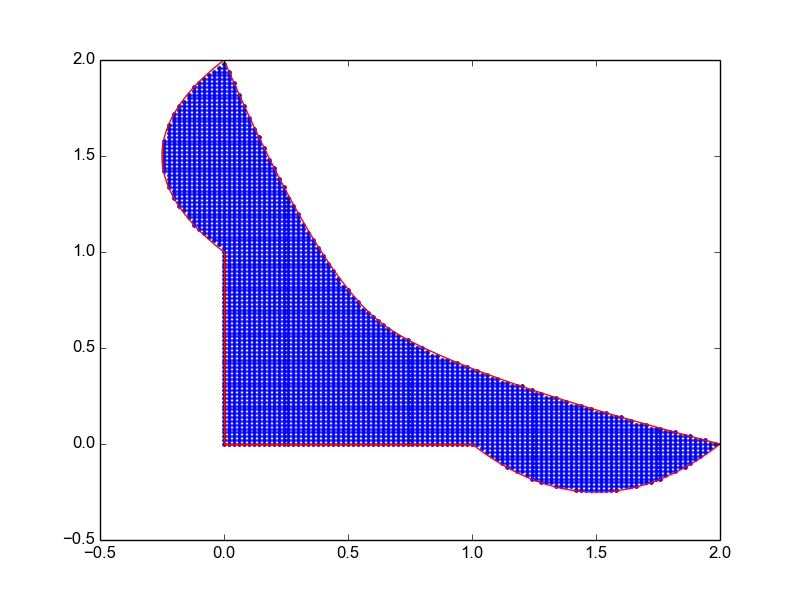
\includegraphics[width=0.5\linewidth]{figure_v_2_h_002.png}
  \hfil \caption{Множество достижимости для системы с V=2, h=0.02}
  \label{fig:v22}

\end{figure}

Для различных значений ресурса $V$ и шага сетки $h$ мы вычислили
расстояние хаусдорфа между теоретичесской оценкой множества
достижимости и тем, что получилось в результате работы
алгоритма. Результаты представлены в табл.~\ref{tab:hsd_ndft}, где в
первой колонке расположены значения ресурса $V$, во второй --- шага
$h$ и в третьей --- расстояния Хаусдорфа. Поскольку этот пример чисто
импульсный, здесь не приводится шаг по времени.Нетрудно заметить, что мы получаем линейный порядок сходимости в
зависимости от шага см рис.~\ref{fig:conv_nd}

\begin{table}[h]
  \centering
  \begin{tabular}{|*{3}{c|}}
    $V$&$h$&$\rho(A,B)$\\ \hline
    1&0.2&0.19357953184\\
    1&0.1&0.0989472244814\\
    1&0.04&0.04\\
    1&0.02&0.02\\
    1&0.01&0.01\\
    2&0.4&0.335023013171\\
    2&0.2&0.193935429287\\
    2&0.08&0.080131031276\\
    2&0.04&0.04\\
    2&0.02&0.02\\
    3&0.6&0.6\\
    3&0.3&0.29644979071\\
    3&0.12&0.130019551125\\
    3&0.06&0.0659015266245\\
    3&0.03&0.0309661912566\\
    5&1.0&1.14082938538\\
    5&0.5&0.5\\
    5&0.2&0.205052066625\\
    5&0.1&0.0985691231869\\
    5&0.05&0.0470656986497\\
    7&1.4&1.89238926658\\
    7&0.7&1.0191890624\\
    7&0.28&0.363069883153\\
    7&0.14&0.139983207703\\
    7&0.07&0.0724479673101\\
  \end{tabular}
  \caption{Расстояние Хаусдорфа в зависимости от шага сетки для
    различных значений ресурса}
  \label{tab:hsd_ndft}
\end{table}

\begin{figure}[h]
  \centering
  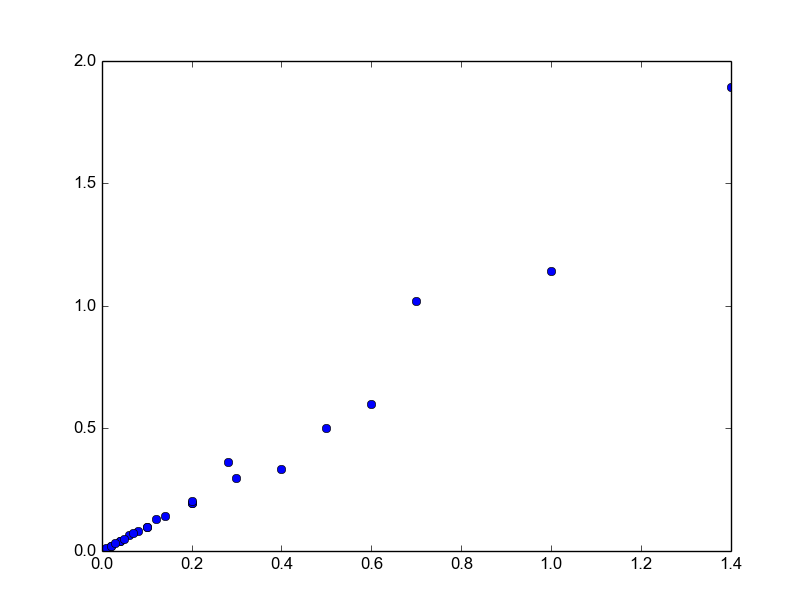
\includegraphics[width=0.5\linewidth]{conv_nd.png}
  \hfil \caption{Зависимость расстояния от шага сетки}
  \label{fig:conv_nd}
\end{figure}


\subsection{Пример системы с дрейфом}
\label{sec:swd}

В следующем примере, присутсвует простой дрейф. Для этого примера
также существует аналитическая оценка границы множества достижимости~\cite{AVS2016}

\begin{equation*}
  \begin{aligned}[b]
    &\dot{x_1}(t) = (1 -x_2(t))v_1(t), & x_1(0)=0\\
    &\dot{x_2}(t) = (1-x_1(t))v_2(t), & x_2(0) = 0\\[8pt]
    &v_1(t) \ge 0, v_2(t) \ge 0 \\
    &\int_{0}^{1} |v_1(t) + v_2(t)| dt \le V
  \end{aligned}
\end{equation*}

На Рис.~\ref{fig:h001_01} Представлено множество достижимости для
такой системы.

\begin{figure}[h]
  \centering
  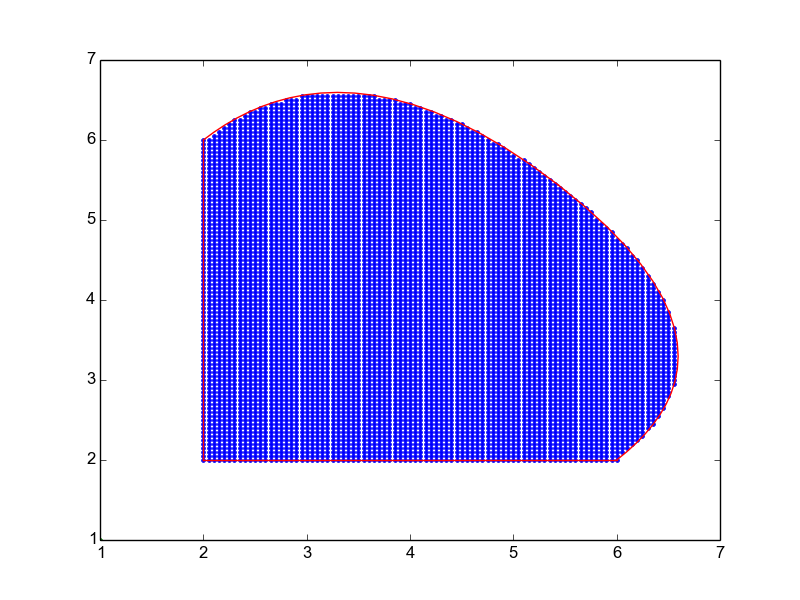
\includegraphics[width=0.5\linewidth]{figure_dc_h_005_ht_02}
  \hfil \caption{Множество достижимости для системы с h=0.05, ht=0.2}
  \label{fig:h001_01}
\end{figure}


В этой системе отклонение считалось для различных значений шага по
времени $h_t$ и шага сетки $h$. Мы вычислили
расстояние хаусдорфа между теоретичесской оценкой множества
достижимости и тем, что получилось в результате работы
алгоритма. Результаты представлены в табл.~\ref{tab:hsd_wdft}, где в
первой колонке расположены значения $h_t$, во второй --- шага
$h$ и в третьей --- расстояния Хаусдорфа. Нетрудно заметить, что здесь
мы также получаем линейный порядок сходимости в
зависимости от шага см рис.~\ref{fig:conv_d}


\begin{table}[h]
  \centering
  \begin{tabular}{|*{3}{c|}}
    $h_t$&$h$&$\rho(A,B)$\\ \hline
    1&0.2&0.217882468317\\
    1&0.1&0.1\\
    1&0.05&0.0474658824842\\
    1&0.01&0.00930483745156\\
    0.5&0.2&0.282842712475\\
    0.5&0.1&0.1\\
    0.5&0.05&0.0474658824842\\
    0.5&0.01&0.00930483745156\\
    0.2&0.2&0.217882468317\\
    0.2&0.1&0.1\\
    0.2&0.05&0.0474658824842\\
    0.2&0.01&0.00930483745156\\
    0.01&0.01&0.00930483745156\\
  \end{tabular}
  \caption{Расстояние Хаусдорфа в зависимости от шага сетки для
    различных значений ресурса}
  \label{tab:hsd_wdft}

\end{table}

\begin{figure}[h]
  \centering
  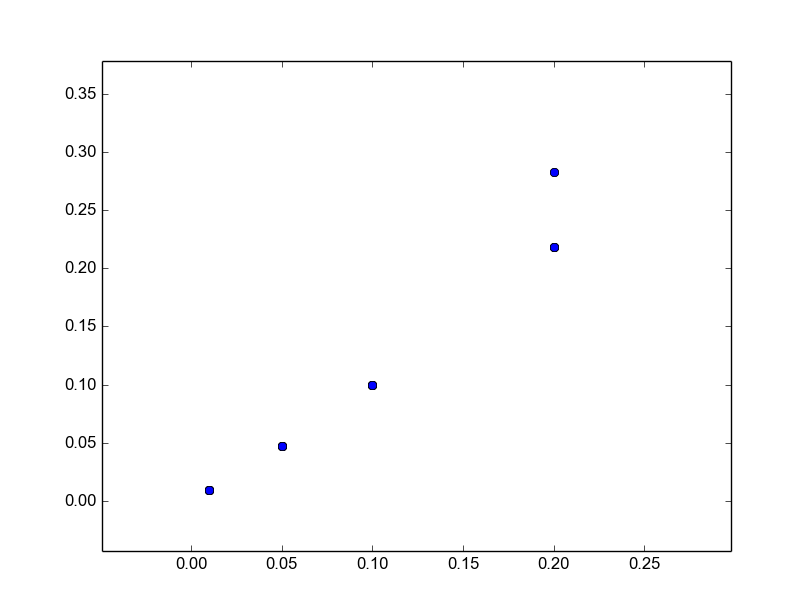
\includegraphics[width=0.5\linewidth]{conv_d.png}
  \hfil \caption{Зависимость расстояния от шага сетки}
  \label{fig:conv_d}
\end{figure}


\subsection{Пример без дрейфа с ограничением}
\label{sec:swdnrsb}
 
Данный пример также является чисто импульсным, как и первый, но с
одним введенными в систему дополнением --- матрица $G(x)$ умжножается
на $2 - x_1^2+ x_2^2$, таким образом система не должна выходить за
пределы круга радиуса $\sqrt{2}$.

\begin{figure}[h]
  \centering
  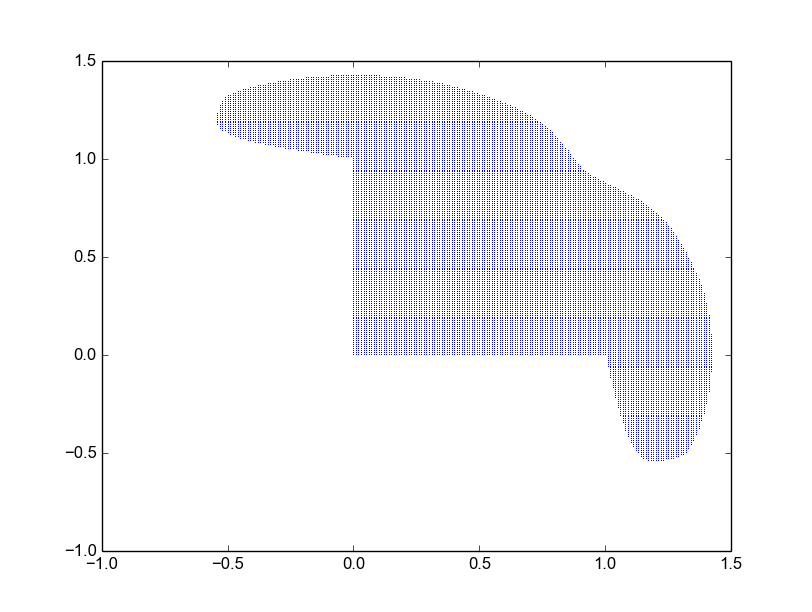
\includegraphics[width=0.5\linewidth]{figure_ndb_v7.png}
  \hfil \caption{Множество достижимости для системы с ограничением}
  \label{fig:vfb}
\end{figure}



\subsection{Пример с неодносвязным множеством достижимости}
\label{sec:swdnrs}


Интегральные кривые этого примера при нулевом управлении
представляют собой окружности с центром в начале координат, причем
фазовая скорость по модулю всюду равена 1. Как и в предыдущем примере,
управления неотрицательны.

\begin{equation*}
  \begin{aligned}[b]
    &\dot{x_1}(t) = \frac{x_2}{\left\|x\right\|} + x_1v_1, &x_1(0) =
    0,\quad v_1(t) \ge 0;\\
    &\dot{x_2}(t) = \frac{-x_1}{\left\|x\right\|} + x_2v_2, &x_2(0)
    = 0,\quad v_2(t) \ge 0.\\
    &\int\limits_0^{13} |v_1(t)| + |v_2(t)| dt \le 1
  \end{aligned}
\end{equation*}
Здесь $\left\| \cdot \right\|$ --- евклидова норма.

Для этого примера условие корректности
Фробениуса выполняется. 
В этом примере матрица $G(x)$ имеет вид 

\begin{equation*}
  G(x) = 
  \begin{pmatrix}
    x_1 & 0 \\
    0 & x_2
  \end{pmatrix}
\end{equation*}
И нетрудно убедиться, что здесь   $[\varphi,\psi] \equiv 0$

На Рис.~\ref{fig:v1h0.02} Представлено множество достижимости для
такой системы.


\begin{figure}[h]
  \centering

  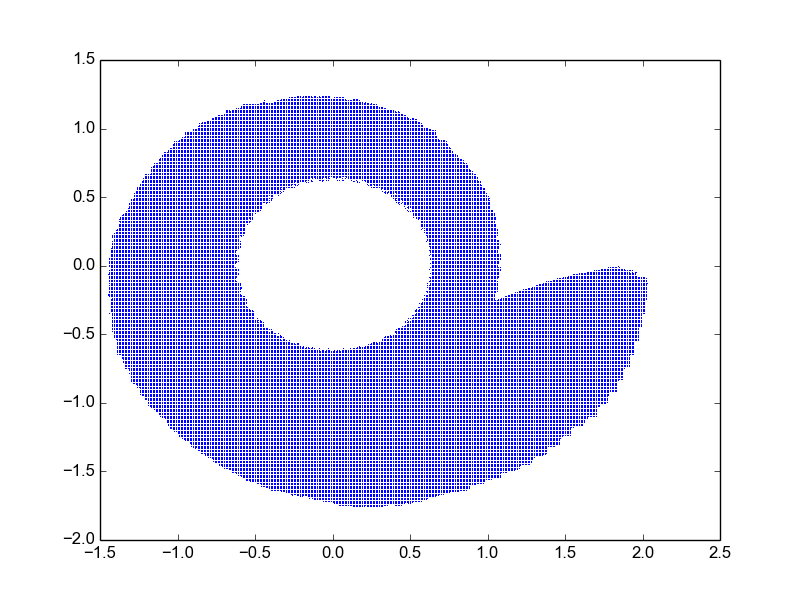
\includegraphics[width=0.5\linewidth]{/figure_d_h_001_ht_01}
  \hfil \caption{Множество достижимости для системы с h=0.01, ht=0.1}
  \label{fig:v1h0.02}
\end{figure}

\section{Программа}
\label{sec:program}

При реализации алгоритма использовался язык программирования python
вместе с библеотекой для научных и инженерных расчетов scipy.

Основу кода состовляет класс \emph{ImpulseSystem}, который хранит
функции $f(x)$ и $G(x)$, позволяя вычислять множество достижимости для
различных начальных данных и параметров времени. 

\begin{verbatim}

def __init__(self, drift=None, impulse=None):
    self.drift = drift
    self.impulse = impulse
    self.x_0 = None
    self.ht = None
    self.h = None
    self.time = None
    self.value = None
    self.cost = dict()
    self.state_space = dict()
    self.grid_error = 0

def integrate(self, x_0, ht, h, time, value):

def impulse_jump(self, points_queue):

def make_drift(self):

def get_costs_at(self, i, j):

def get_cost(self, cur_matrix, x, y):
\end{lstlisting}

Принци работы весьма прост. Мы создаем экземпляр класса
\emph{ImpulseSystem} отдавая ему в конструктор функции отвечающие за
дрейф --- \emph{drift} и импульсное воздействие ---
\emph{impulse}. Например для первого примера \ref{sec:snwd}. Созданный объект будет
выглядеть следующим образом:

\begin{lstlisting}[language=Python,
caption={Интерфейс Impulse System}]
F = None
G = lambda x: sc.matrix([[1 - x[1], 0], [0, 1 - x[0]]])
isys = ImpulseSystem(drift=F, impulse=G)
\end{verbatim}

Для запуска процесса интегрирования мы вызываем метод
\emph{integrate}. На вход которому подаем все параметры --- точку
$x_0$, шаг по времени $h_t$, шаг по сетке $h$, время $T$ и ресурс $V$.

Общий процесс идет по принципу, что описан выше смотри
\ref{sec:wave_alg}. На каждом интервале сначала работает метод
\emph{impulse jump}, затем все полученные точки дрейфуют под действием
\emph{make drift} и так для всех интервалов.

После завершения работы программы мы получаем список точек, для
аппрокисмации множества достижимости.

\section*{Заключение}
\label{sec:conclusion}

В дипломной работе были рассмотрены два алгоритма аппроксимации множеств
достижимости для импульсных управляемых систем с билинейной структурой.
Алгоритмы реализованы в среде Scientific Python; выполнен ряд численных
экспериментов; проведено сравнение с аналитическими оценками множества
достижимости в тех случаях, когда это возможно; найдена погрешность алгоритма
(расстояние Хаусдорфа между множеством достижимости и его аппроксимацией). На
основе полученных данных сделаны следующие выводы:

1) Переборный алгоритм может быть применен лишь для грубой аппроксимации в
наиболее простых случаях (размерность 1-2), поскольку объем вычислений
экспоненциально зависит от числа участков, на которые разбит временной
интервал.

2) Даже в относительно простых примерах время работы пиксельного алгоритма на
1-2 порядка меньше, чем у переборного.

3) Пиксельный метод для систем с билинейной структурой весьма эффективен:
погрешность алгоритма во всех рассмотренных случаях близка к шагу разбиения
фазового пространства.

Следует отметить, что в рамках дипломной работы данные алгоритмы применялись к
довольно узкому классу задач. Некоторые расширения этого класса (отсутствие
ограничения на знак управлений) не требуют существенной переработки алгоритмов
и программ. Изменение нормы, в которой задано ограничение на векторное
управление, приведет к заметному усложнению алгоритма.

Требует дальнейшего исследования вопрос об эффективном выборе дискретизации
фазового пространства:  целесообразно измельчать сетку в окрестности множества,
на котором функция цены не дифференцируема.
\pagebreak
\begin{thebibliography}{99}
        \addcontentsline{toc}{section}{Список литературы}

    \bibitem{DS2011} { Dykhta~V.A., Samsonyuk~O.N.}  Some applications of
        Hamilton-Jacobi inequalities for classical and impulsive optimal
        control problems // European Journal of Control. Nonsmooth analysis,
        Control and Optimization. 2011. Vol.17. Pp. 55--69.

    \bibitem{ZS1991} { Завалищин С.Т., Сесекин А.Н.}  {Импульсные
        процессы: модели и приложения}.  М.: Наука, 1991.

    \bibitem{MR2005} { Миллер Б.М., Рубинович Е.Я.}  { Оптимизация
        динамических систем с импульсными управлениями}.  М.: Наука, 2005.

    \bibitem{DS2003} { Дыхта В.А., Самсонюк О.Н.}  Оптимальное импульсное
        управление с приложениями.  М.: Физматлит, 2003.

    \bibitem{SS2010} { Самсонюк~О.Н., Сесекин~А.Н.} Оценки и свойства
        интегральных воронок траекторий нелинейных импульсных систем //
        Тез. докл. II Международной школы-семинара «Нелинейный анализ и
        экстремальные задачи». Иркутск, ИДСТУ СО РАН, 28 июня -- 4 июля 2010
        г. 2010. С. 64--65.

    \bibitem{BS2005} Вдовина О.И., Сесекин А.Н. Численное построение
        областей достижимости для систем с импульсными управлениями //
        Тр. Ин-та математики и механики УрО РАН.  2005. Т. 11, № 1.

    \bibitem{FM2011} Т. Ф. Филиппова, О. Г. Матвийчук, Алгоритмы
        оценивания множеств достижи- мости импульсных управляемых систем с
        эллипсоидальными фазовыми ограничениями, Автомат. и телемех.,
        2011, выпуск 9, 127–141

    \bibitem{G1997} Гурман В.И. Принцип расширения в задачах
        управления. 2-е изд., перераб. и доп. М.:Физматлит, 1997, 288 с.

    \bibitem{M1993} Миллер Б.М. Метод разрывной замены времени в задачах
        оптимального управления импульсными и дискретно-непрерывными
        системами // Автоматика и телемеханика. 1993. № 12. С. 3--32.

    \bibitem{MR1995} Motta M., Rampazzo F. Space-time trajectories of
        nonlinear systems driven by ordinary and impulsive controls //
        Differential Integral Equations. 1995. Vol. 8.  Pp. 269-288.

    \bibitem{MS1999} Motta M., Sartori C. Discontinuous solutions to
        unbounded differential inclusions under state constraints.
        Applications to optimal control problems // Set-Valued
        Analysis. 1999. Vol. 7. Pp. 295-322.

    \bibitem{WZ2007} Wolenski P.R., Zabic S.  A Sampling Method and
        Approximation Results for Impulsive Systems // SIAM J. Control
        Optim., 2007, Vol. 46. Pp. 983-998.

    \bibitem{AVS2016} {Апанович Д. В.,Воронов В. А.,Самсонюк О. Н.},
        Построение множества достижимости двумерной импульсной управляемой
        системы с билинейной структурой// Изв. Иркутского
        гос. ун-та. Сер. Математика, 15 (2016), 3–16

    \bibitem{AV2015_1} Апанович Д.В., Воронов В.А. Численная аппроксимация
        множеств достижимости нелинейных импульсных управляемых систем. //
        Теория управления и математическое моделирование: Тезисы докладов
        Всероссийской конференции с международным участием, посвященной
        памяти профессора Н. В. Азбелева и профессора Е. Л. Тонкова (Ижевск,
        Россия, 9–11 июня 2015 г.). Ижевск: Изд-во «Удмуртский университет»,
        2015. С. 24-25.

    \bibitem{AV2015_2} Апанович Д.В., Воронов В.А. Численная аппроксимация
        неодносвязного множества достижимости нелинейной импульсной
        управляемой системы. //  Тезисы докладов III Российско-монгольской
        конференции молодых ученых по математическому моделированию,
        вычислительно-информационным технологиям и управлению (Иркутск
        (Россия) – Ханх (Монголия), 23 июня – 30 июня 2015 г.). – Иркутск:
        Научно-организационный отдел ИДСТУ СО РАН, 2015. С. 17.


    \bibitem{DS2000} {Дыхта В. А., Самсонюк О.Н.} Оптимальное импульсное
        управление с приложениями. — М.: ФИЗМАТ ЛИТ, 2000. — 256 с. — ISBN
        5-9221-0097-1.

    \bibitem{S1999} {J.A. Sethian.} Level Set Methods and Fast Marching Methods: evolving
        interfaces in computational geometry, computer vision and matherial
        science. — 2nd Ed. — Cambridge Univ. Press, 1999

\end{thebibliography}

\pagebreak
\section*{Приложения}
\label{sec:appl}

\normalsize
\subsection*{Приложение 1}
\label{appl_src}

\begin{verbatim}
__author__ = 'dvapan'

import scipy as sc
from scipy.integrate import odeint
from scipy.linalg import norm
import logging
import matplotlib.pyplot as plt


delta = [(0, 1), (1, 0), (0, -1), (-1, 0)]


class ImpulseSystem(object):
    drift = None
    impulse = None

    def __init__(self, drift=None, impulse=None):
        self.drift = drift
        self.impulse = impulse
        self.x_0 = None
        self.ht = None
        self.h = None
        self.time = None
        self.value = None
        self.cost = dict()
        self.state_space = dict()
        self.logger = logging.getLogger('rs_counter.ImpulseSystem')
        self.logger.info('create ImpulseSystem object')
        self.grid_error = 0

    def integrate(self, x_0, ht, h, time, value):
        self.x_0 = x_0
        self.ht = ht
        self.h = h
        self.time = time
        self.value = value
        i, j = 0, 0
        points_queue = set([(i, j)])
        self.state_space[i, j] = 1.0 * value
        self.logger.info('start integrate system')
        if self.drift:
            for t in sc.arange(0, time, ht):
                self.logger.info('t = {0}'.format(t))
                self.impulse_jump(points_queue)
                self.make_drift()
                points_queue = set(self.state_space.keys())
        self.impulse_jump(points_queue)

    def impulse_jump(self, points_queue):
        self.logger.info('start making impulse jump')

        h = self.h

        counter = 1
        divider = (self.value * 1 / self.h) ** 2
        while points_queue:
            cur_point = points_queue.pop()
            i, j = cur_point
            if counter % divider == 0:
                self.logger.info('Working at {0} = {1} | iteration {2}'.format((i, j), self.state_space[i, j], counter))
            if not self.cost.get((i, j)):
                self.cost[i, j] = self.get_costs_at(i, j)
            for k in range(len(delta)):
                dx, dy = delta[k]
                c = self.cost[i, j][k]
                new_v = self.state_space[i, j] - c * h
                if new_v > 0 and self.state_space.get((i + dx, j + dy), 0) < new_v:
                    self.state_space[i + dx, j + dy] = new_v
                    points_queue.add((i + dx, j + dy))
            counter += 1

    def make_drift(self):
        self.logger.info('start making drift')
        next_lay = dict()
        dt = self.ht  # 1.0 * self.time / self.nt
        # logger.info("{0}".format(dt))
        h = self.h

        for (i, j) in self.state_space.keys():
            x, y = sc.array([i, j]) * h + self.x_0
            nx = sc.array(odeint(self.drift, (x, y), sc.linspace(0, dt, 10))[-1])
            #logger.info("{0} --> {1}".format((x, y), nx))
            new_i, new_j = map(int, (map(round, (nx - self.x_0) / h)))

            new_error = norm(sc.array([self.x_0[0] + i * h, self.x_0[1] + j * h]) - nx)

            next_lay[new_i, new_j] = self.state_space[i, j]
        self.state_space = next_lay

    def get_costs_at(self, i, j):
        h = self.h
        cur_matrix = self.impulse((self.x_0[0] + i * h, self.x_0[1] + j * h))
        return [self.get_cost(cur_matrix, 0, 1),
                self.get_cost(cur_matrix, 1, 0),
                self.get_cost(cur_matrix, 0, -1),
                self.get_cost(cur_matrix, -1, 0)]

    def get_cost(self, cur_matrix, x, y):
        try:
            v = sc.linalg.solve(cur_matrix, (x, y))
            if v[0] >= 0 and v[1] >= 0:
                return norm(v)
            else:
                return sc.NAN
        except:
            if cur_matrix[0, 0] == 0.0 and cur_matrix[1, 1] != 0.0:
                v = y / cur_matrix[1, 1]
                if v > 0:
                    return v
            if cur_matrix[1, 1] == 0.0 and cur_matrix[0, 0] != 0.0:
                v = x / cur_matrix[0, 0]
                if v > 0:
                    return v
            return sc.NAN


def get_part_hausdorphe(bp, points):
    return max(map(lambda p: min(map(lambda q: norm(p - q),
                                     points)),
                   sc.array(bp).transpose()))


def test_sample_without_drift(h,V):
    plt.clf()
    x_0 = [0, 0]
    F = None
    G = lambda x: sc.matrix([[1 - x[1], 0], [0, 1 - x[0]]])
    isys = ImpulseSystem(drift=F, impulse=G)
    isys.integrate(x_0, None, h, None, V)
    points = []
    bp = []
    for (i, j) in isys.state_space.keys():
        points.append([x_0[0] + i * h, x_0[1] + j * h])
    points = sc.array(points)
    sc.save('out/points_v_{0}_h_{1}'.format(V, h), points)
    logger.info('plotting approximated reachability set')
    if h <= 0.01 or V >= 5:
        plt.plot(points[:, 0], points[:, 1], ',')
    else:
        plt.plot(points[:, 0], points[:, 1], '.')
    logger.info('count Hausdorff distance')

    a = sc.linspace(0, 1, max(1.0/h, 100))
    plt.plot(sc.zeros(len(a)), a, 'r')
    bp.append(get_part_hausdorphe([sc.zeros(len(a)), a], points))
    logger.info('current distance {0}'.format(max(bp)))
    plt.plot(a, sc.zeros(len(a)), 'r')
    bp.append(get_part_hausdorphe([a, sc.zeros(len(a))], points))
    logger.info('current distance {0}'.format(max(bp)))

    a = sc.linspace(0, V, max(1.0/h, 100))
    r = 1 - sc.exp(-a / 2)
    y = r + (V - a) * (1 - r)
    plt.plot(r, y, 'r')
    bp.append(get_part_hausdorphe([r, y], points))
    logger.info('current distance {0}'.format(max(bp)))

    plt.plot(y, r, 'r')
    bp.append(get_part_hausdorphe([y, r], points))
    logger.info('current distance {0}'.format(max(bp)))
    if V > 1:
        if V <= 3:
            a = sc.linspace(V/2, V, max(1.0/h, 100))
        else:
            a = sc.linspace(V/4, V/2, max(1.0/h, 100))

        plt.plot(a, (1 - a) * (V - a), 'r')
        bp.append(get_part_hausdorphe([a, (1 - a) * (V - a)], points))
        logger.info('current distance {0}'.format(max(bp)))

        plt.plot((1 - a) * (V - a), a, 'r')
        bp.append(get_part_hausdorphe([(1 - a) * (V - a), a], points))
        logger.info('current distance {0}'.format(max(bp)))
    if V > 2:
        a = sc.linspace(0, V-2,  max(1.0/h, 100))
        r = sc.exp(a/2)
        plt.plot(1 - r, 1+r+(V-2-a)*r, 'r')
        bp.append(get_part_hausdorphe([1-r, 1+r+(V-2-a)*r], points))
        logger.info('current distance {0}'.format(max(bp)))
        plt.plot(1-r-(V-2-a)*r, 1 + r, 'r')
        bp.append(get_part_hausdorphe([1-r-(V-2-a)*r,1+r], points))
        logger.info('current distance {0}'.format(max(bp)))
        plt.plot(1+r+(V-2-a)*r, 1 - r, 'r')
        bp.append(get_part_hausdorphe([1+r+(V-2-a)*r, 1 - r], points))
        logger.info('current distance {0}'.format(max(bp)))
        plt.plot(1 + r, 1-r-(V-2-a)*r, 'r')
        bp.append(get_part_hausdorphe([1 + r, 1-r-(V-2-a)*r], points))
        logger.info('current distance {0}'.format(max(bp)))
    res = max(bp)
    f = open('out/data', 'a')
    f.write("{0} {1} {2}\n".format(V, h, res))
    f.close()
    plt.savefig("out/figure_v_{0}_h_{1}.png".format(V, h))
    #plt.show()


def test_sample_with_drift(h, ht):
    V = 1
    T = 13
    plt.clf()
    x_0 = [2, 0]
    G = lambda x: sc.matrix([[-x[0], 0], [0, -x[1]]])
    F = lambda x, t: [x[1]/sc.sqrt(x[1]**2+x[0]**2), -x[0]/sc.sqrt(x[1]**2+x[0]**2)]
    logger.info('count RS for h = {0}, ht = {1}'.format(h, ht))
    isys = ImpulseSystem(drift=F, impulse=G)
    isys.integrate(x_0, ht, h, T, V)
    points = []
    for (i, j) in isys.state_space.keys():
        points.append([x_0[0] + i * h, x_0[1] + j * h])
    points = sc.array(points)
    logger.info('count testable RS')
    isys2 = ImpulseSystem(drift=F, impulse=G)
    isys2.integrate(x_0, ht, h/2.0, T, V)
    points2 = []
    for (i, j) in isys2.state_space.keys():
        points2.append([x_0[0] + i * h, x_0[1] + j * h])
    points2 = sc.array(points2)
    
    logger.info('count Hausdorff distance')
    error = 0
    for p in points:
        min_h = min(map(lambda x: norm(x-p), points2))
        logger.info('min dist for point {0} = {1}. Current distance {2}'.format(p, min_h,error))
        if min_h>error:
            error = min_h
    
    sc.save('out/points_d_v_{0}_h_{1}'.format(V, h), points)
    logger.info('plotting approximated reachability set')
    if h < 0.05:
        plt.plot(points[:, 0], points[:, 1], ',')
    else:
        plt.plot(points[:, 0], points[:, 1], '.')
    # f = open('out/data', 'a')
    # f.write("{0} {1} {2}\n".format(ht, h, error))
    # f.close()
    plt.savefig("out/figure_d_h_{0}_ht_{1}.png".format(h, ht))


def test_sample_with_drift_counted(h,ht):
    V = 2
    T = 1
    plt.clf()
    x_0 = [1, 1]
    G = lambda x: sc.matrix([[x[1], 0], [0, x[0]]])
    #G = lambda x: sc.matrix([[0, 0], [0, 0]])
    F = lambda x, t: [1,1]
    logger.info('count RS for h = {0}, ht = {1}'.format(h, ht))
    isys = ImpulseSystem(drift=F, impulse=G)
    isys.integrate(x_0, ht, h, T, V)
    points = []
    bp = []
    for (i, j) in isys.state_space.keys():
        points.append([x_0[0] + i * h, x_0[1] + j * h])
    points = sc.array(points)
    logger.info('plotting approximated reachability set')
    if h < 0.05:
        plt.plot(points[:, 0], points[:, 1], ',')
    else:
        plt.plot(points[:, 0], points[:, 1], '.')
    f = open('log1.txt')
    s = f.read()
    lines = s.split('\r\n')[:-2]
    data = sc.array([map(float, l.split('    ')[1:]) for l in lines]).transpose()
    plt.plot(data[0,:-21], data[1,:-21],'r')
    plt.plot(data[0,21:], data[1,21:],'r')
    bp.append(get_part_hausdorphe([data[0,:], data[1,:]], points))
    x = sc.linspace(2,6,40)
    y = sc.full(len(x), 2)
    bp.append(get_part_hausdorphe([x,y], points))
    bp.append(get_part_hausdorphe([y,x], points))
    plt.plot(1,1,'.')
    plt.plot(x, y, 'r')
    plt.plot(y, x, 'r')
    res = max(bp)
    f = open('out/data', 'a')
    f.write("{0} {1} {2}\n".format(ht, h, res))
    f.close()
    sc.save('out/points_dc_ht_{0}_h_{1}'.format(ht, h), points)
    plt.savefig("out/figure_dc_h_{0}_ht_{1}.png".format(h, ht))


if __name__ == "__main__":
    logger = logging.getLogger('rs_counter')
    logger.setLevel(logging.DEBUG)
    # create file handler which logs even debug messages
    fh = logging.FileHandler('out/script.log')
    fh.setLevel(logging.DEBUG)
    # create console handler with a higher log level
    ch = logging.StreamHandler()
    ch.setLevel(logging.DEBUG)
    # create formatter and add it to the handlers
    formatter = logging.Formatter('%(asctime)s - %(name)s - %(levelname)s - %(message)s')
    fh.setFormatter(formatter)
    ch.setFormatter(formatter)
    # add the handlers to the logger
    logger.addHandler(fh)
    logger.addHandler(ch)

    seg_num = 100
    x_0 = [0, 0]

    ht=None
    h=0.01
    T=None
    V = 7
    F = None
    G = lambda x: sc.matrix([[-(1 - x[1])*(x[0]**2 + x[1]**2 - 2), 0], [0, -(1 - x[0])*(x[0]**2 + x[1]**2 - 2)]])
    isys = ImpulseSystem(drift=F, impulse=G)
    isys.integrate(x_0, ht, h, T, V)
    points = []
    bp = []
    for (i, j) in isys.state_space.keys():
        points.append([x_0[0] + i * h, x_0[1] + j * h])
    points = sc.array(points)
    logger.info('plotting approximated reachability set')
    if h < 0.05:
        plt.plot(points[:, 0], points[:, 1], ',')
    else:
        plt.plot(points[:, 0], points[:, 1], '.')
    plt.show()
    G = lambda x: sc.matrix([[-x[0], 0], [0, -x[1]]])
    F = lambda x, t: [x[1]/sc.sqrt(x[1]**2+x[0]**2), -x[0]/sc.sqrt(x[1]**2+x[0]**2)]
    f = open('out/data', 'w')
    f.write('ht,h,hausd_dist\n')
    f.close()
    V = 7
    test_sample_without_drift(V/10.0, V)

    for V in [1,2,5,7]:
        for h in [V/5.0, V/10.0, V/25.0, V/50.0, V/100.0]:
            logger.info('Start testing sample: V = {0}, h = {1}'.format(V, h))
            test_sample_without_drift(h, V)
    for ht in [1, 0.5, 0.2, 0.01]:
        for h in [0.2, 0.1, 0.05, 0.01]:
            logger.info('Start testing sample: ht = {0}, h = {1}'.format(ht, h))
            test_sample_with_drift_counted(h, ht)

    test_sample_with_drift(0.01, 0.1)

\end{verbatim}

\end{document}

